\section{Auswertung}
\label{sec:Auswertung}

\subsection{Bestimmung von $U_0$ und $R_i$ der Monozelle}

Es wird die Klemmspannung $U_k$ in Abhängigkeit des Stromes $I$ gemessen. 
Die aufgenommenen Werte sind in Tabelle \ref{tab:Monozelle} aufgeführt. 

\begin{table}
\centering
\caption{Spannungs- und Stromwerte der Monozelle}
\label{tab:Monozelle}
\sisetup{table-format=2.1}
\begin{tabular}{c c}
\toprule
$U_k \,/\, \si{\volt}$ & $I \,/\, \si{\milli\ampere}$\\
\midrule
1.550 & 25.0\\
1.525 &  27.5\\
1.500 &  31.0\\
1.450 &  38.0\\
1.425 &  46.0\\
1.400 &  49.5\\
1.350 &  57.0\\
1.300 &  61.5\\
1.250 &  77.5\\
1.200 &  85.0\\
1.100 & 110.0\\
0.700 & 175.0\\
0.450 & 215.0\\
0.400 & 225.0\\
\bottomrule
\end{tabular}
\end{table}

\subsection{Bestimmung von $U_0$ und $R_i$ der Monozelle 
            mit Gegenspannung}
\begin{table}
  \centering
  \caption{Spannungs- und Stromwerte der Monozelle unter 
           Gegenspannung}
  \label{tab:Gegen}
  \sisetup{table-format=2.1}
  \begin{tabular}{c c}
    \toprule
     $U_k \,/\, \si{\volt}$ & $I \,/\, \si{\milli\ampere}$\\
    \midrule
      1.900 &  40.0\\
      1.925 &  42.0\\
      1.950 &  45.5\\
      1.975 &  52.5\\
      2.000 &  55.5\\
      2.050 &  65.0\\
      2.100 &  73.0\\
      2.150 &  82.5\\
      2.200 &  90.0\\
      2.250 & 101.0\\
      2.300 & 105.0\\
      2.400 & 120.0\\
      2.500 & 140.0\\
      2.700 & 170.0\\
      3.000 & 220.0\\
    \bottomrule
  \end{tabular}
\end{table}


\begin{figure}
  \centering
  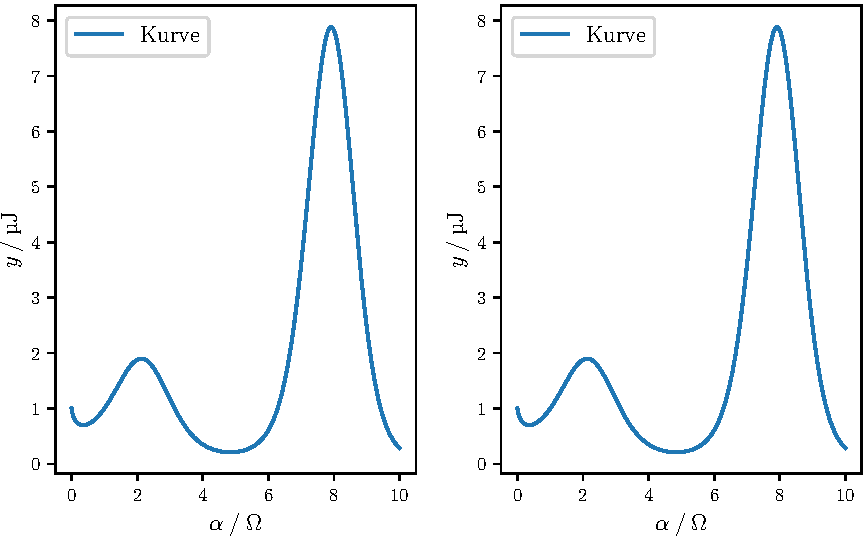
\includegraphics{plot.pdf}
  \caption{Plot.}
  \label{fig:plot}
\end{figure}

\subsection{Bestimmung von $U_0$ und $R_i$ des Rechteckausgangs
            eines RC-Generators}
  \begin{table}
    \centering
    \caption{Spannungs- und Stromwerte der Rechteckspannung}
    \label{tab:Rechteck}
    \sisetup{table-format=2.1}
    \begin{tabular}{c c}
      \toprule
       $U_k \,/\, \si{\volt}$ & $I \,/\, \si{\milli\ampere}$\\
      \midrule
        0.54 & 2.15\\
        0.52 & 2.50\\
        0.50 & 2.85\\
        0.48 & 3.25\\ 
        0.46 & 3.65\\
        0.42 & 4.55\\
        0.38 & 5.20\\
        0.35 & 5.80\\
        0.30 & 6.75\\
        0.25 & 7.7\\
        0.20 & 8.55\\
      \bottomrule
    \end{tabular}
  \end{table}


\subsection{Bestimmung von $U_0$ und $R_i$ des Sinusausgangs
            eines RC-Generators}
  \begin{table}
    \centering
    \caption{Spannungs- und Stromwerte der Sinusspannung}
    \label{tab:Sinus}
    \sisetup{table-format=2.1}
    \begin{tabular}{c c}
      \toprule
       $U_k \,/\, \si{\volt}$ & $I \,/\, \si{\milli\ampere}$\\
      \midrule
        2.100 & 0.355\\
        2.000 & 0.600\\
        1.900 & 0.650\\
        1.800 & 0.850\\
        1.750 & 0.950\\
        1.700 & 1.050\\
        1.650 & 1.100\\
        1.600 & 1.200\\
        1.550 & 1.275\\
        1.500 & 1.350\\
        1.450 & 1.425\\
        1.400 & 1.500\\
        1.375 & 1.575\\
        1.300 & 1.650\\
        1.250 & 1.725\\
        1.000 & 2.125\\
        0.750 & 2.550\\
      \bottomrule
    \end{tabular}
  \end{table}